\documentclass[9pt,a5paper,twoside]{extarticle}

\usepackage[inner=13mm,outer=11mm,top=13mm,bottom=15mm,headheight=12pt]{geometry}
\usepackage[T1]{fontenc}
\usepackage[utf8]{inputenc}
\usepackage{tgheros}
\renewcommand{\familydefault}{\sfdefault}
\usepackage[table]{xcolor}
\usepackage{graphicx}
\usepackage{tikz}
\usepackage{tabularx}
\usepackage{booktabs}
\usepackage{enumitem}
\usepackage{microtype}
\usepackage{fancyhdr}
\usepackage{tcolorbox}
\tcbuselibrary{breakable,skins}
\usepackage{hyperref}
\usepackage{xurl}
\graphicspath{{./}{consortium/workshop-materials/}{../../news/open-call/}{news/open-call/}}

\definecolor{Night}{HTML}{071A2B}
\definecolor{DeepBlue}{HTML}{123B5D}
\definecolor{Sky}{HTML}{3D8EAF}
\definecolor{Aqua}{HTML}{6EC5CB}
\definecolor{Gold}{HTML}{E5AD55}
\definecolor{Mist}{HTML}{EDF5F7}
\definecolor{Cloud}{HTML}{F7FAFB}
\definecolor{Ink}{HTML}{142632}
\definecolor{Muted}{HTML}{526775}
\definecolor{Divider}{HTML}{CAD9DE}
\definecolor{Coral}{HTML}{D9785C}
\definecolor{Violet}{HTML}{7A5BA7}
\definecolor{Teal}{HTML}{2E7D6E}
\definecolor{PaleBlue}{HTML}{92B6D5}
\definecolor{Ochre}{HTML}{B98548}
\definecolor{Slate}{HTML}{65747D}
\definecolor{Magenta}{HTML}{C85A89}

\hypersetup{
  colorlinks=true,
  linkcolor=DeepBlue,
  urlcolor=DeepBlue,
  pdftitle={Workshop Participant Booklet, Version 1.1 — Accelerating Astrophysical Discovery with Foundation Models},
  pdfauthor={Accelerating Astrophysical Discovery consortium},
  pdfsubject={Lorentz Center workshop, 14--18 September 2026},
  pdfkeywords={Version 1.1, 14 September 2026}
}

\newcommand{\bookletversion}{VERSION 1.1}
\newcommand{\bookletdate}{14 SEPTEMBER 2026}

\color{Ink}
\setlength{\parindent}{0pt}
\setlength{\parskip}{4pt}
\setlist[itemize]{leftmargin=4mm,itemsep=2pt,topsep=2pt}
\setlist[enumerate]{leftmargin=5mm,itemsep=2pt,topsep=2pt}
\emergencystretch=1.5em

\pagestyle{fancy}
\fancyhf{}
\fancyhead[LE]{\scriptsize\color{Muted}ACCELERATING ASTROPHYSICAL DISCOVERY}
\fancyhead[RO]{\scriptsize\color{Muted}PARTICIPANT BOOKLET · SEPTEMBER 2026}
\fancyfoot[C]{\scriptsize\color{Muted}\bookletversion\ · \bookletdate}
\fancyfoot[LE,RO]{\scriptsize\color{Muted}\thepage}
\renewcommand{\headrulewidth}{0pt}
\renewcommand{\footrulewidth}{0pt}

\newcommand{\eyebrow}[1]{%
  {\small\bfseries\color{Sky}\MakeUppercase{#1}}\par\vspace{2mm}}

\newcommand{\pagetitle}[2]{%
  \eyebrow{#1}%
  {\fontsize{20}{22}\selectfont\bfseries\color{Night}#2\par}%
  \vspace{3mm}%
  {\color{Gold}\rule{18mm}{1.4pt}}\par\vspace{4mm}}

\newcommand{\chartdot}[1]{%
  \tikz[baseline=-0.45ex]{\fill[#1] (0,0) circle[radius=1.05mm];}}

\newtcolorbox{infobox}[1][]{
  enhanced,
  colback=Mist,
  colframe=Mist,
  boxrule=0pt,
  borderline west={2.2pt}{0pt}{Sky},
  arc=1.5mm,
  left=3.5mm,right=3.5mm,top=3mm,bottom=3mm,
  #1
}

\newtcolorbox{darkbox}[1][]{
  enhanced,
  colback=Night,
  colframe=Night,
  coltext=white,
  boxrule=0pt,
  arc=1.5mm,
  left=4mm,right=4mm,top=3.5mm,bottom=3.5mm,
  #1
}

\newtcolorbox{guidebox}[1]{
  enhanced,
  colback=Cloud,
  colframe=Divider,
  boxrule=.5pt,
  borderline north={1.8pt}{0pt}{Sky},
  arc=1.5mm,
  left=3.5mm,right=3.5mm,top=3mm,bottom=3mm,
  title={#1},
  coltitle=DeepBlue,
  fonttitle=\bfseries,
  attach title to upper={\par\vspace{1.5mm}}
}

\newcommand{\dayheader}[4]{%
  \eyebrow{#1 · #3}%
  {\fontsize{18}{20}\selectfont\bfseries\color{Night}#2\par}%
  \vspace{2.5mm}
  \begin{infobox}
    \textbf{Deliverable}\quad #4
  \end{infobox}
  \vspace{2mm}
}

\newcommand{\slot}[3]{%
  \textbf{#1} & \textbf{#2}\if\relax\detokenize{#3}\relax\else\par\vspace{-1pt}{\scriptsize\color{Muted}#3}\fi\\
  \arrayrulecolor{Divider}\midrule
}

\newenvironment{scheduletable}{%
  \renewcommand{\arraystretch}{1.16}%
  \rowcolors{2}{Cloud}{white}%
  \tabularx{\linewidth}{@{\hspace{1mm}}>{\raggedright\arraybackslash\color{DeepBlue}}p{23mm} >{\raggedright\arraybackslash}X@{\hspace{1mm}}}
  \rowcolor{DeepBlue}\color{white}\bfseries Time & \color{white}\bfseries Session\\
  \arrayrulecolor{DeepBlue}\midrule
}{%
  \endtabularx
}

\begin{document}

% Cover
\thispagestyle{empty}
\hypersetup{pageanchor=false}
\begin{tikzpicture}[remember picture,overlay]
  \fill[Night] (current page.south west) rectangle (current page.north east);
  \node[anchor=north,inner sep=0pt] at (current page.north) {%
    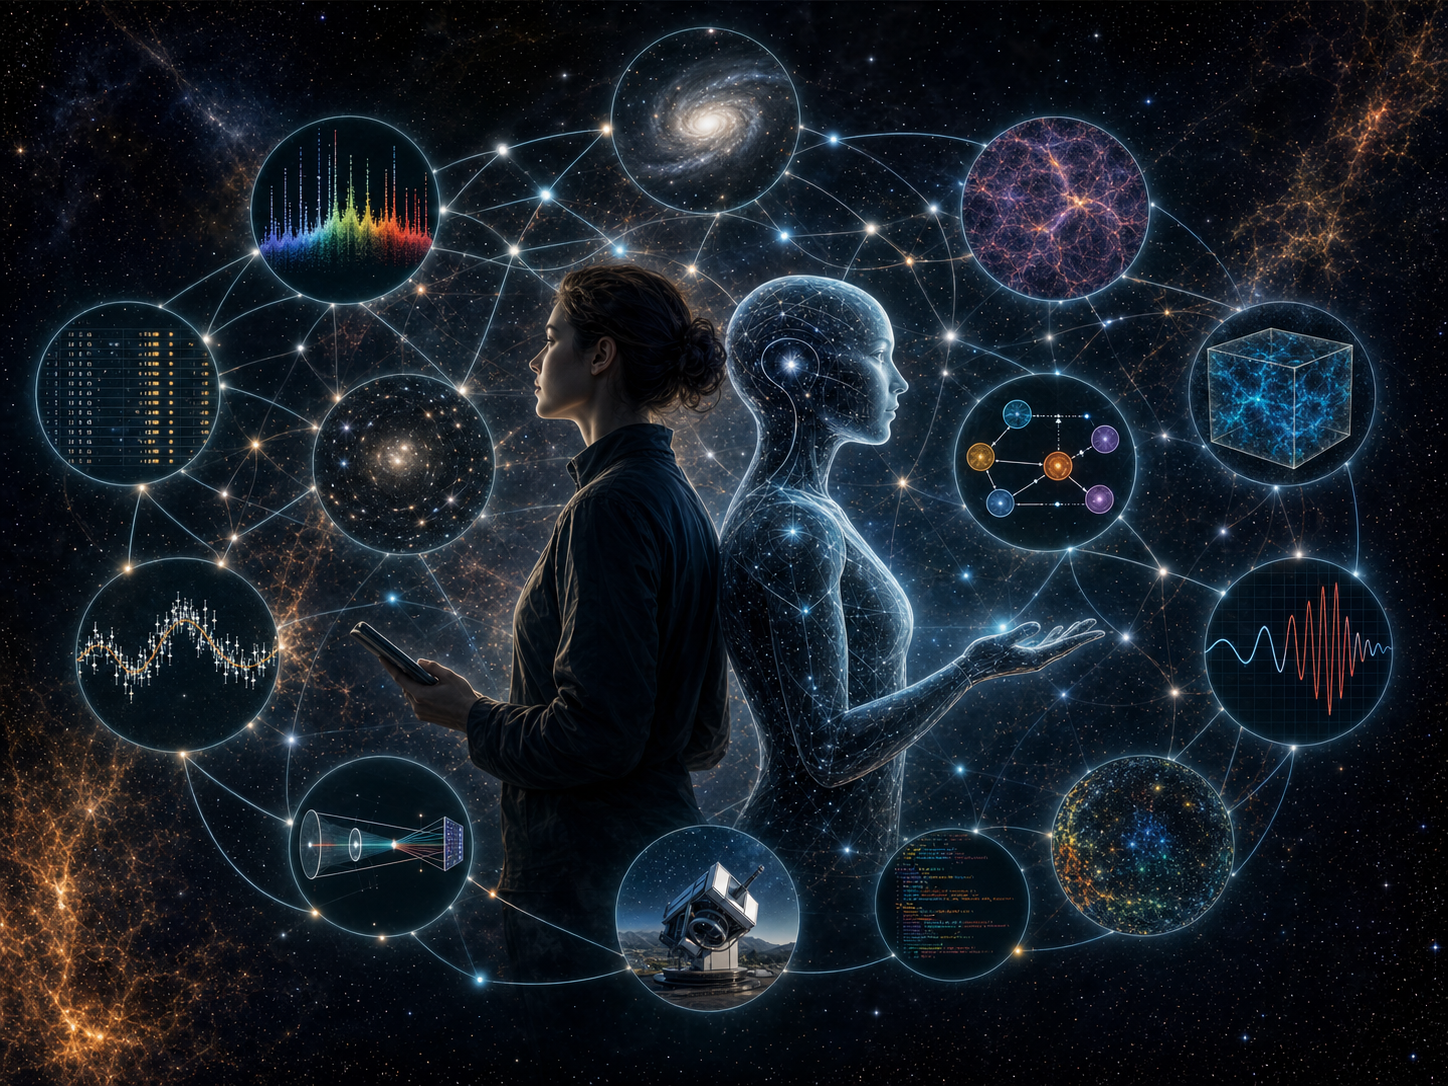
\includegraphics[width=\paperwidth]{joint-human-ai-discovery.png}};
  \fill[shade,left color=Night!95,right color=DeepBlue!92]
    (current page.south west) rectangle ([yshift=-104.8mm]current page.north east);
  \node[anchor=north west,text width=124mm,align=left]
    at ([xshift=12mm,yshift=-112mm]current page.north west) {%
      {\small\bfseries\color{Aqua}LORENTZ CENTER WORKSHOP\par}
      \vspace{4mm}
      {\fontsize{24}{27}\selectfont\bfseries\color{white}
        Accelerating Astrophysical\par Discovery\par}
      \vspace{1mm}
      {\fontsize{15}{18}\selectfont\color{white!86}
        with Foundation Models\par}
      \vspace{5mm}
      {\large\bfseries\color{Gold}Participant booklet\par}
      \vspace{4mm}
      {\small\color{white!86}14--18 September 2026\quad·\quad Leiden, The Netherlands\par}
      \vspace{2.5mm}
      {\scriptsize\bfseries\color{Aqua}\bookletversion\ · \bookletdate\par}
    };
\end{tikzpicture}
\null\newpage

\setcounter{page}{1}
\hypersetup{pageanchor=true}
\pagetitle{Welcome}{A week built for making}

Dear Lorentz Workshop participant,

This booklet introduces the consortium's ambition and relevancy graph, lays out the working timetable, and suggests a few things to bring into the week. Bring concrete examples, informed questions, and a willingness to build across disciplinary boundaries.

\begin{darkbox}
  {\bfseries\color{Gold}AT A GLANCE}\par\vspace{2mm}
  \begin{tabularx}{\linewidth}{@{}>{\bfseries\color{Aqua}}p{25mm}X@{}}
    Workshop & Accelerating Astrophysical Discovery with Foundation Models\\[2mm]
    Dates & Monday 14 to Friday 18 September 2026\\[2mm]
    Venue & Lorentz Center@omega, Leiden, The Netherlands\\[2mm]
    Start times & Monday at 10:00; Tuesday--Friday at 9:30\\
  \end{tabularx}
\end{darkbox}

\vspace{4mm}
\begin{infobox}
  {\bfseries\color{DeepBlue}CONTINUE WITH THE CONSORTIUM}\par\vspace{2mm}
  Visit the \href{https://accelerating-astrophysical-discovery.github.io/}{consortium website} for workshop materials, news, and ongoing work.

  Interested in taking part? \href{https://docs.google.com/forms/d/e/1FAIpQLSf9cepUblJ_UEt2-9TlchmWkx-JINSjlTbjsOd1VkEH4i9W2Q/viewform}{Join the consortium} through the same sign-up form linked from the members page.
\end{infobox}

\newpage

\eyebrow{Workshop community}
{\fontsize{18}{20}\selectfont\bfseries\color{Night}List of participants\par}
\vspace{1.5mm}
{\color{Gold}\rule{18mm}{1.4pt}}\par\vspace{2mm}

{\scriptsize
\setlength{\tabcolsep}{1.2mm}
\renewcommand{\arraystretch}{0.84}
\rowcolors{2}{Cloud}{white}
\begin{tabularx}{\linewidth}{@{\hspace{1mm}}>{\bfseries\color{DeepBlue}}l l >{\raggedright\arraybackslash}X@{\hspace{1mm}}}
  \rowcolor{DeepBlue}\color{white}\bfseries Last name & \color{white}\bfseries First name & \color{white}\bfseries Affiliation\\
  Albert & Joshua G. & California Institute of Technology\\
  Albin & Thomas & Freelancer Scientist\\
  Angeloudi & Eirini & University of Hamburg, Germany\\
  Bester & Hertzog Landman & SARAO, South Africa\\
  Bhihe & Cedric & BSC, Spain\\
  Callingham & Joseph & ASTRON/UvA\\
  Cañas-Herrera & Guadalupe & Leiden Observatory\\
  Caron & Sascha & Radboud University\\
  Cheng & Ting-Yun & University of Groningen\\
  Ciuca & Ioana & Stanford University, USA\\
  Cruz & Marcos & Instituto de Física de Cantabria, Spain\\
  Cuesta Lazaro & Carolina & Flatiron Institute / New York University\\
  De la Torre Luque & Pedro & Universidad Autónoma de Madrid (UAM)\\
  Eckner & Christopher & Instituto de Astrofísica de Canarias\\
  Fernández Sopuerta & Carlos & ICE/CSIC, Spain\\
  Hartman & Nicole & MIT / IAIFI\\
  Heng & Ik Siong & University of Glasgow, UK\\
  Huertas-Company & Marc & IAC\\
  Huppenkothen & Daniela & University of Amsterdam, The Netherlands\\
  Jain & Divesh & University of Heidelberg\\
  Keenan & Ryan & Max Planck Institute for Astronomy\\
  Keller & Christoph & National Solar Observatory\\
  Khan & Sebastian & Starling Bank\\
  Leonhard & David & University of Bonn\\
  Li & Youyou & GRAPPA, University of Amsterdam\\
  Lopez & Melissa & Nikhef\\
  Loukili & Soulaymane & BSC, Spain\\
  Madireddy & Sandeep & Simons SkAI, Argonne National Laboratory\\
  Pérez Romero & Judit & IFIC (UV/CSIC)\\
  Portegies Zwart & Simon & Leiden Observatory\\
  Poux--Bouret & Benjamin & LIRA, Observatoire de Paris, PSL, Sorbonne, Paris Cité, CY Cergy Paris Université, CNRS\\
  Ruiz de Austri & Roberto & Universidad de Valencia\\
  Sáinz-Pardo Díaz & Judith & Spanish National Research Council (CSIC) -- Institute of Physics of Cantabria (IFCA)\\
  Samia & Noelle & Simons SkAI\\
  Smirnov & Oleg & Rhodes University \& SARAO\\
  Smith & Michael & Harvard-Smithsonian Center for Astrophysics\\
  Sotoudeh & Hadi & University of Cambridge\\
  Stevance & Héloïse & Oxford University, UK\\
  Tallada Crespí & Pau & CIEMAT-PIC\\
  Vacheret & Antonin & Laboratoire Corpusculaire de Caen UMR 6534, Caen, France\\
  Villaescusa-Navarro & Francisco & Simons Foundation\\
  Weigel & Philip & Harvard University\\
  Zaharijas & Gabrijela & University of Nova Gorica\\
  Zhao & Yue & SURF, NL\\
\end{tabularx}
}

\vspace{3mm}
\begin{tcolorbox}[enhanced,colback=Cloud,colframe=Divider,boxrule=.5pt,arc=1.5mm,left=3.5mm,right=3.5mm,top=2.5mm,bottom=2.5mm]
  {\small\bfseries\color{DeepBlue}Consortium fields}\hfill
  {\scriptsize\color{Muted}Share of field entries}\par\vspace{1.5mm}
  \begin{minipage}[c]{0.34\linewidth}
    \centering
    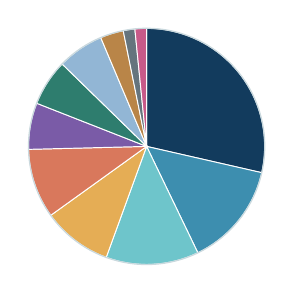
\begin{tikzpicture}
      \path[fill=DeepBlue,draw=white,line width=.35pt] (0,0) -- (90:15mm) arc[start angle=90,end angle=-12.857,radius=15mm] -- cycle;
      \path[fill=Sky,draw=white,line width=.35pt] (0,0) -- (-12.857:15mm) arc[start angle=-12.857,end angle=-64.286,radius=15mm] -- cycle;
      \path[fill=Aqua,draw=white,line width=.35pt] (0,0) -- (-64.286:15mm) arc[start angle=-64.286,end angle=-110,radius=15mm] -- cycle;
      \path[fill=Gold,draw=white,line width=.35pt] (0,0) -- (-110:15mm) arc[start angle=-110,end angle=-144.286,radius=15mm] -- cycle;
      \path[fill=Coral,draw=white,line width=.35pt] (0,0) -- (-144.286:15mm) arc[start angle=-144.286,end angle=-178.571,radius=15mm] -- cycle;
      \path[fill=Violet,draw=white,line width=.35pt] (0,0) -- (-178.571:15mm) arc[start angle=-178.571,end angle=-201.429,radius=15mm] -- cycle;
      \path[fill=Teal,draw=white,line width=.35pt] (0,0) -- (-201.429:15mm) arc[start angle=-201.429,end angle=-224.286,radius=15mm] -- cycle;
      \path[fill=PaleBlue,draw=white,line width=.35pt] (0,0) -- (-224.286:15mm) arc[start angle=-224.286,end angle=-247.143,radius=15mm] -- cycle;
      \path[fill=Ochre,draw=white,line width=.35pt] (0,0) -- (-247.143:15mm) arc[start angle=-247.143,end angle=-258.571,radius=15mm] -- cycle;
      \path[fill=Slate,draw=white,line width=.35pt] (0,0) -- (-258.571:15mm) arc[start angle=-258.571,end angle=-264.286,radius=15mm] -- cycle;
      \path[fill=Magenta,draw=white,line width=.35pt] (0,0) -- (-264.286:15mm) arc[start angle=-264.286,end angle=-270,radius=15mm] -- cycle;
      \draw[Divider,line width=.45pt] (0,0) circle[radius=15mm];
    \end{tikzpicture}
  \end{minipage}\hfill
  \begin{minipage}[c]{0.62\linewidth}
    {\fontsize{6.9}{7.8}\selectfont
    \renewcommand{\arraystretch}{0.96}
    \begin{tabularx}{\linewidth}{@{}c>{\raggedright\arraybackslash}X>{\bfseries\color{DeepBlue}}r@{}}
      \chartdot{DeepBlue} & AI & 28.6\%\\
      \chartdot{Sky} & Cosmology & 14.3\%\\
      \chartdot{Aqua} & Radio & 12.7\%\\
      \chartdot{Gold} & Computational physics & 9.5\%\\
      \chartdot{Coral} & Gravitational waves & 9.5\%\\
      \chartdot{Violet} & Gamma-rays & 6.3\%\\
      \chartdot{Teal} & Neutrinos & 6.3\%\\
      \chartdot{PaleBlue} & Optical & 6.3\%\\
      \chartdot{Ochre} & X-Ray & 3.2\%\\
      \chartdot{Slate} & CRs & 1.6\%\\
      \chartdot{Magenta} & Infrared & 1.6\%\\
    \end{tabularx}}
  \end{minipage}
\end{tcolorbox}
\newpage

\pagetitle{The consortium}{Two connected pillars}

\begin{tcolorbox}[enhanced,colback=DeepBlue,colframe=DeepBlue,coltext=white,boxrule=0pt,arc=2mm,left=5mm,right=5mm,top=5mm,bottom=5mm]
  {\large\bfseries\color{Gold}PILLAR 01}\par\vspace{2mm}
  {\Large\bfseries Design science for human--AI collaboration}\par\vspace{3mm}
  The first goal is to design how future astrophysicists and cosmologists will do science in collaboration with AI. This is more than adding chat interfaces to existing tools. It means redesigning workflows so humans, reasoning language models, simulators, archives, instruments, and foundation models can jointly form hypotheses, retrieve evidence, run checks, update beliefs, and communicate results.
\end{tcolorbox}

\vspace{4mm}

\begin{tcolorbox}[enhanced,colback=Mist,colframe=Mist,boxrule=0pt,arc=2mm,left=5mm,right=5mm,top=5mm,bottom=5mm,borderline west={2.5pt}{0pt}{Gold}]
  {\large\bfseries\color{Sky}PILLAR 02}\par\vspace{2mm}
  {\Large\bfseries\color{Night}Build a joint representation of physical data}\par\vspace{3mm}
  The second goal is to build the technical substrate: a model that learns across observations, simulations, synthetic observations, language, code, and instrumental context. It should support meaningful embeddings for retrieval and serendipity, along with generative capabilities for conditional inference across linked views of the same physical system.
\end{tcolorbox}

\vfill
\begin{infobox}
  \textbf{One shared ambition.} The two pillars meet in an agentic discovery system: reasoning models guide scientific work, the joint-representation model grounds that work in physical evidence, and humans remain responsible for judgement.
\end{infobox}
\newpage

\pdfbookmark[1]{The relevancy graph}{relevancy-graph}
\pagetitle{Training structure}{The relevancy graph}

\begin{center}
  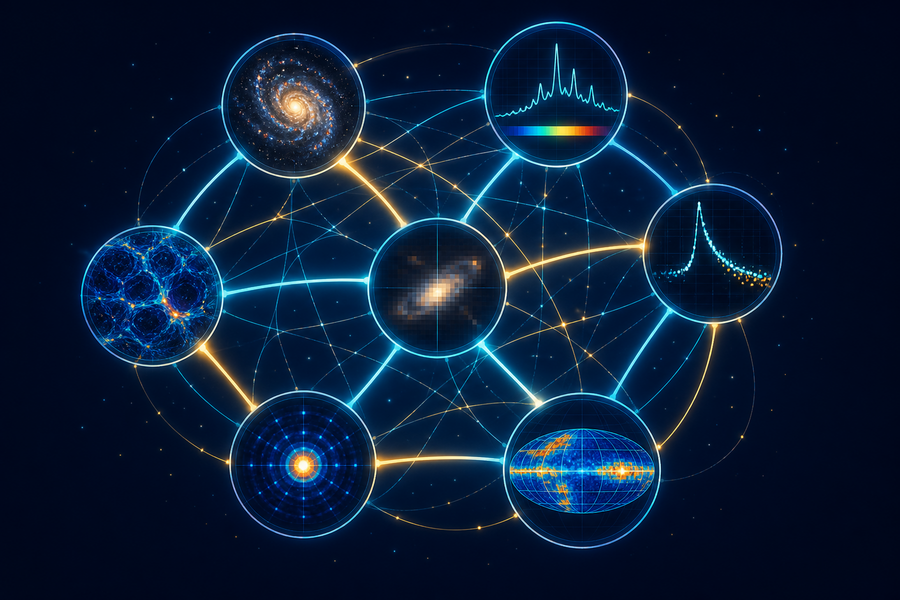
\includegraphics[width=.82\linewidth]{relevancy-graph.png}
\end{center}

\vspace{4mm}
\begin{darkbox}
  {\bfseries\color{Gold}FROM DATA RELATIONSHIPS TO ATTENTION}\par\vspace{2mm}
  We envision a large graph database whose nodes are physical data and whose links encode relevancy. An astrophysical system, for example, can be observed repeatedly by different instruments in different modalities and simulated by different codes.

  During self-supervised training, sampled graph connectivity forms the attention mask. Text naturally supplies an autoregressive order; physical data admit a more general attentional field---cross-modal, many-to-many, and hierarchical. The model uses this context to predict or reconstruct withheld data.
\end{darkbox}

\vfill
{\small\color{Muted}Nodes are physical data. Relevancy links define which data may exchange information during training.}
\newpage

\pagetitle{Before Leiden}{Bring ingredients,\\not finished answers}

\begin{tcolorbox}[enhanced,colback=DeepBlue,colframe=DeepBlue,coltext=white,boxrule=0pt,arc=2mm,left=5mm,right=5mm,top=4.5mm,bottom=4.5mm]
  {\large\bfseries\color{Gold}ASTROPHYSICS + COMPUTATIONAL PHYSICS}\par\vspace{2mm}
  Think about use cases where AI could help humans study the cosmos and do better science if it could understand, reason about, and generate physical data.

  Prepare a list of astrophysical data you can access. Any modality is welcome, including:
  \begin{itemize}[label=\textcolor{Aqua}{\textbullet}]
    \item observations, catalogues, spectra, images, time series, and event lists;
    \item simulation code, snapshots, initial conditions, and synthetic observations;
    \item multimodal observations of the same systems;
    \item instrument responses, calibration context, uncertainties, and provenance.
  \end{itemize}
\end{tcolorbox}

\vspace{4mm}
\begin{tcolorbox}[enhanced,colback=Mist,colframe=Mist,boxrule=0pt,arc=2mm,left=5mm,right=5mm,top=4.5mm,bottom=4.5mm,borderline west={2.5pt}{0pt}{Gold}]
  {\large\bfseries\color{DeepBlue}AI + COMPUTATIONAL INFRASTRUCTURE}\par\vspace{2mm}
  Think about the architectural challenges facing a joint-representation model that must learn deep, self-supervised representations of large physical datasets.

  Also consider the infrastructure required to train across physical datasets that can dwarf the data used to train language models:
  \begin{itemize}[label=\textcolor{Sky}{\textbullet}]
    \item long context, heterogeneous tokenisation, and shared latent spaces;
    \item compute-to-data training across distributed archives and HPC systems;
    \item data access, preprocessing, provenance, monitoring, and validation;
    \item staged scaling, simulator-backed synthetic data, and failure modes.
  \end{itemize}
\end{tcolorbox}

\vfill
{\small\color{Muted}If you span both groups, bring both perspectives. If you span neither exactly, bring the constraints, examples, and questions from your own domain.}
\newpage

\pagetitle{The week}{The week at a glance}

\renewcommand{\arraystretch}{1.22}
\begin{tabularx}{\linewidth}{@{}>{\bfseries\color{DeepBlue}}p{20mm} >{\raggedright\arraybackslash}p{38mm} >{\raggedright\arraybackslash}X@{}}
  \toprule
  Day & Focus & Main deliverable\\
  \midrule
  Monday & Vocabulary, use cases, evaluation & Use cases and evaluation criteria\\
  \addlinespace[1mm]
  Tuesday & Parallel work: data + model & First tests of data and model hypotheses and interfaces\\
  \addlinespace[1mm]
  Wednesday & Parallel work: data + model & Reviewed evidence and hypotheses ready to implement\\
  \addlinespace[1mm]
  Thursday & AI-assisted hypothesis implementation & Working hypotheses implemented in code with AI assistance\\
  \addlinespace[1mm]
  Friday & Roadmap, governance, funding & Roadmap\\
  \bottomrule
\end{tabularx}

\vspace{5mm}
\begin{darkbox}
  {\bfseries\color{Gold}THE HAND-OFF}\par\vspace{2mm}
  Monday establishes the scientific use cases for everyone. On Tuesday and Wednesday, technical work proceeds in two parallel tracks: \textbf{Data} (relevancy graph, representation, and tokenisation) and \textbf{Model} (architecture, training, and physical alignment). Wednesday reviews evidence and prepares the hypotheses for implementation. Thursday implements working hypotheses in code with AI assistance. Friday turns the week's results into a roadmap.
\end{darkbox}

\vfill
{\small\color{Muted}Formal working hours are 10:00--16:30 on Monday, 9:30--17:00 Tuesday--Thursday, and 9:30--13:30 on Friday. The building is open for arrivals and coffee from 09:00 on Monday.}
\newpage

\pdfbookmark[1]{Consortium workstreams}{consortium-workstreams}
\pagetitle{Working together}{Consortium workstreams}

{\small
\renewcommand{\arraystretch}{1.2}
\begin{tabularx}{\linewidth}{@{}>{\raggedright\arraybackslash\bfseries\color{DeepBlue}}p{40mm} >{\raggedright\arraybackslash}X@{}}
  \toprule
  Workstream & Working focus\\
  \midrule
  Scientific use cases & Workflows, required functionality, and evaluation targets.\\
  \addlinespace[2mm]
  Data, relevancy graph, tokenisation, and representation & Linked data, typed relationships, provenance, and encodings that preserve physical information.\\
  \addlinespace[2mm]
  Architecture, training, and physical alignment (RLSF) & Model hypotheses, learning objectives, generated states, simulation feedback, and discriminating tests.\\
  \addlinespace[2mm]
  Infrastructure and prototyping & Data-local compute, sampling, software, and runnable components.\\
  \addlinespace[2mm]
  Project oversight & Dependencies, decisions, priorities, milestones, and ownership.\\
  \addlinespace[2mm]
  Network and funding & Expertise, partners, resources, funding, and sustainable participation.\\
  \bottomrule
\end{tabularx}}

\vspace{3mm}
\begin{infobox}
  \textbf{Stay connected}\quad Share artifacts, evidence, open questions, and requests in plenary. Use public GitHub Issues for non-sensitive coordination and decisions. Human-review AI summaries; keep credentials and restricted information private.
\end{infobox}
\newpage

\pdfbookmark[1]{Monday}{day-monday}
\pagetitle{Monday · 10:00--16:30}{Timetable}

\begin{guidebox}{Purpose of the day}
  Define scientific use cases and evaluation criteria that guide the rest of the week.
\end{guidebox}

\begin{scheduletable}
  \slot{09:00--10:00}{Arrival and coffee}{}
  \slot{10:00--10:30}{Kickoff talk}{}
  \slot{10:30--12:00}{Science 2.0 and use cases}{}
  \slot{12:00--13:30}{Lunch}{}
  \slot{13:30--14:30}{Group synthesis}{}
  \slot{14:30--15:00}{Coffee break}{}
  \slot{15:00--16:30}{Evaluation targets and workstream planning}{}
  \slot{16:30 onward}{Welcome reception}{}
\end{scheduletable}

\vfill
\begin{infobox}
  \textbf{Keep asking}\quad What would count as evidence that this workflow produces better science, rather than simply more output?
\end{infobox}
\newpage

\pdfbookmark[1]{Tuesday}{day-tuesday}
\pagetitle{Tuesday · 9:30--17:00}{Timetable}

\begin{guidebox}{Purpose of the day}
  Develop and test hypotheses in two parallel tracks: \textbf{Data} (relevancy graph, representation, and tokenisation) and \textbf{Model} (architecture, training, and physical alignment).
\end{guidebox}

\begin{scheduletable}
  \slot{9:30--10:00}{Vocabulary and hypotheses kickoff}{}
  \slot{10:00--10:30}{Parallel workstreams}{}
  \slot{10:30--11:00}{Coffee break}{}
  \slot{11:00--12:00}{Parallel workstreams}{}
  \slot{12:00--13:30}{Lunch}{}
  \slot{13:30--14:30}{Group synthesis}{}
  \slot{14:30--15:00}{Coffee break}{}
  \slot{15:00--17:00}{Parallel workstreams}{}
\end{scheduletable}

\vfill
\begin{infobox}
  \textbf{Keep asking}\quad What could we make or test now, and what does another team need from us?
\end{infobox}
\newpage

\pdfbookmark[1]{Wednesday}{day-wednesday}
\pagetitle{Wednesday · 9:30--17:00}{Timetable}

\begin{guidebox}{Purpose of the day}
  Review the evidence, continue the parallel Data and Model work, and prepare selected hypotheses for implementation.
\end{guidebox}

\begin{scheduletable}
  \slot{9:30--10:00}{Progress and experimental-results review}{}
  \slot{10:00--10:30}{Parallel workstreams}{}
  \slot{10:30--11:00}{Coffee break}{}
  \slot{11:00--12:00}{Parallel workstreams}{}
  \slot{12:00--13:30}{Lunch}{}
  \slot{13:30--14:30}{Group synthesis}{}
  \slot{14:30--15:00}{Coffee break}{}
  \slot{15:00--17:00}{Parallel workstreams}{}
  \slot{17:00--20:00}{Workshop dinner}{}
\end{scheduletable}
\newpage

\pdfbookmark[1]{Thursday}{day-thursday}
\pagetitle{Thursday · 9:30--17:00}{Timetable}

\begin{guidebox}{Purpose of the day}
  Implement selected hypotheses in code with AI assistance and test what the implementations demonstrate.
\end{guidebox}

\begin{scheduletable}
  \slot{9:30--10:00}{Organiser briefing and overnight review}{}
  \slot{10:00--10:30}{Implementation planning}{}
  \slot{10:30--11:00}{Coffee break}{}
  \slot{11:00--12:00}{AI-assisted implementation I}{}
  \slot{12:00--13:30}{Lunch}{}
  \slot{13:30--14:30}{AI-assisted implementation II}{}
  \slot{14:30--15:00}{Coffee break}{}
  \slot{15:00--16:15}{Show-and-tell and integration}{}
  \slot{16:15--17:00}{Closeout and Friday handoff}{}
\end{scheduletable}

\vfill
{\small\color{Muted}\textbf{Thursday rule:} every artifact should connect to a use case, a model capability, and an evaluation target.}
\newpage

\pdfbookmark[1]{Friday}{day-friday}
\pagetitle{Friday · 9:30--13:30}{Timetable}

\begin{guidebox}{Purpose of the day}
  Turn the week's results, open questions, ownership, and resource needs into a roadmap.
\end{guidebox}

\begin{scheduletable}
  \slot{9:30--10:00}{Review of the week}{}
  \slot{10:00--10:30}{Roadmap group discussion}{}
  \slot{10:30--11:00}{Coffee break}{}
  \slot{11:00--11:30}{Funding opportunities}{}
  \slot{11:30--12:00}{Roadmap synthesis}{}
  \slot{12:00--13:30}{Closing lunch}{}
\end{scheduletable}

\vspace{4mm}
\begin{darkbox}
  {\bfseries\color{Gold}PRACTICAL MATTERS}\par\vspace{2mm}
  Discounted hotel reservations are limited, so please book as soon as possible if you need accommodation.

  For practical questions or help with accommodation, contact Maria Krebbers at
  \href{mailto:acceleratingastrophysical@lorentzcenter.nl}{acceleratingastrophysical@lorentzcenter.nl}.
\end{darkbox}

\vfill
\begin{center}
  {\small\bfseries\color{DeepBlue}accelerating-astrophysical-discovery.github.io}\par
  \vspace{2mm}
  {\scriptsize\color{Muted}Bring a use case. Bring a constraint. Leave with something we can build together.}
\end{center}

\end{document}
